% Diskussion L1
% Relative Fehler L1:
% rel. T+ L1:               0,0442+/-0,0033 
% rel. omega+ L1:           0,0423+/-0,0030 
% rel. T- L1:               0,0442+/-0,0033 
% rel. omega- L1:           0,0423+/-0,0030 
% rel. T_S L1:              0,02+/-0,06 
% rel. omega_S L1:          -0,0423+/-0,0030 (nicht mit omega=2pi*(1/T))
% rel. omega_S L1 test:     -2,02+/-0,06 (mit 2pi*(1/T), aber omega_theo ist negativ)
% rel. omega_S L1 test2:    0,02+/-0,06 (ergibt eig am meisten Sinn, mit 2pi*(1/T), aber mit abs(omega_theo))
% Diskussion L2   
% Relative Fehler L2:   
% rel. T+ L2:               0,033+/-0,006
% rel. omega+ L2:           0,034+/-0,006
% rel. T- L2:               0,033+/-0,006
% rel. omega- L2:           0,034+/-0,006
% rel. T_S L2:              0,01+/-0,08
% rel. omega_S L2:          -0,034+/-0,006 (nicht mit omega=2pi*(1/T))
% rel. omega_S L2 test:     -1,99+/-0,08 (mit 2pi*(1/T), aber omega_theo ist negativ)
% rel. omega_S L2 test2:    0,01+/-0,08 (ergibt eig am meisten Sinn, mit 2pi*(1/T), aber mit abs(omega_theo))
\section{Diskussion}
\label{sec:Diskussion}
$$\text{rel. Abweichung} = \frac{\abs(\text{exp. Wert} - \text{theo. Wert})}{\text{theo. Wert}}$$
\section{Originaldaten}
\label{sec:Originaldaten}
% \begin{figure}[H]
%   \centering
%   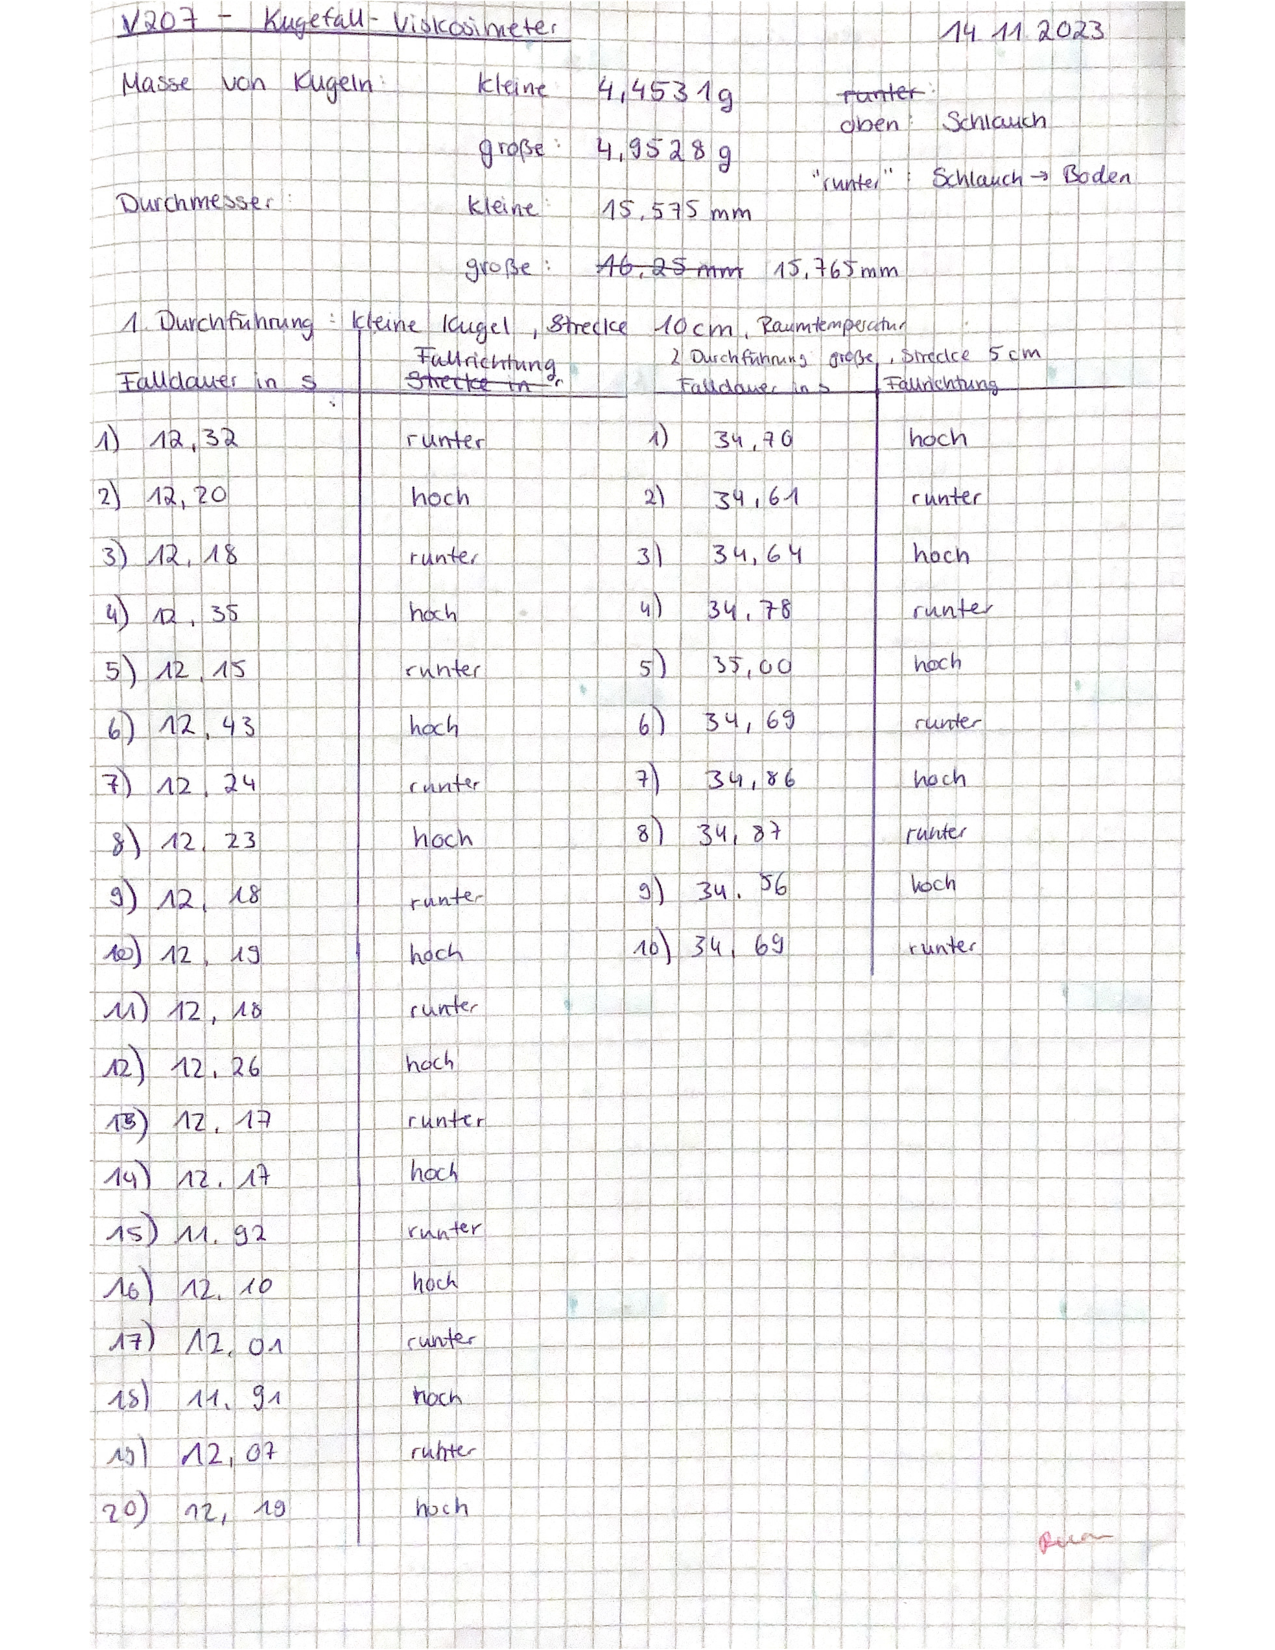
\includegraphics[width=\textwidth]{Messwerte.pdf}
%   \label{fig:Messungen}
% \end{figure}